\chapter{Evaluation}
\label{ch:evaluation}
To evaluate this multi-robot system, we used Gazebo to create a simulated office environment. There were no obstacles to this office environment. Simulation time was used in Gazebo. The simulation time flowed fluctuates, and its flow rate was about 10\%-20\% slower than in real-time. In the experiment, the sensor measured the opening and closing of the door. An open door meant the office was occupied, and a closed-door meant the office was empty and not occupied. The robot gathered measurement data from sensors while running tasks and sent task results and measurement data to the centralized pool. The centralized pool was the global controller that received information about the robots and the environment and made decisions base on the information. The task results and measurement data were counted and analyzed. Two kinds of experiments were designed: gathering information experiments and navigation experiments. Each gathering information experiment ran for 20 simulated minutes. The centralized pool could get about 30 task results and 90-140 measurement data. In each navigation experiment, robots completed 15 navigation tasks. The centralized pool could get 30-60 measurement data. The multi-robot system ran 600 experiments, took about 10,800 simulated minutes, completed 9,000 tasks, and gathered 50,000 measurement data. 

\section{Simulation}

Simulation is essential because it can pre-estimate the performance of the multi-robot system before applying it to a real office environment.
Gazebo is a 3D robot simulator software based on physics simulation. 
To evaluate this multi-robot system, Gazebo was used to create a simulated office environment. The sensors are simulated using a ROS node called ``sensor simulator'' because ROS nodes can use ROS build-in messaging system.

\subsection{Sensor Simulation}
\label{sec:sensor_simulation}

\paragraph{Sensor simulator generated measurement data.}
The measurement data about door status was an integer that could be set to 0 (door closed)or 1 (door opened). The sensor simulator first uses the current simulated timestamp to find the door open probability in the door open probability table. Then generate this number based on this probability. For example, on Monday (day of week value is 2) at simulated time ``10:30:00'' (on time slot 10:00:00-10:59:59), in 80\% probability a ``door open'' was generated and in 20\% a ``door closed'' was generated (Initialized probability of door open was 0.80).

\begin{figure}
\centering
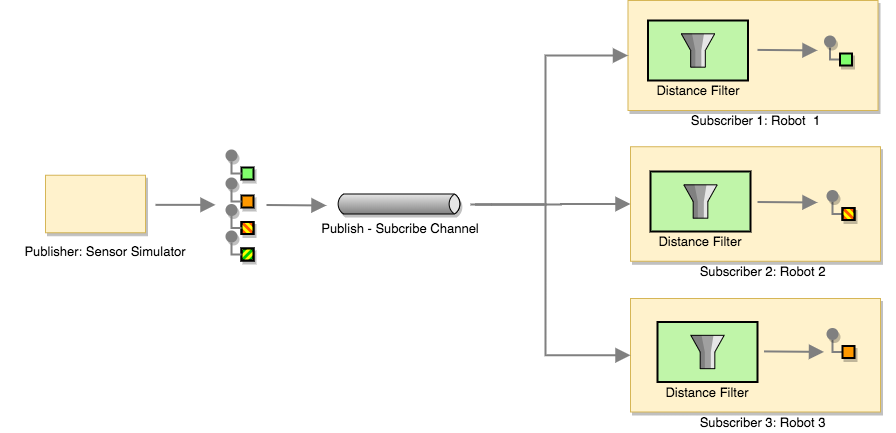
\includegraphics[width = 0.7\textwidth]{content/images/ch4/sensor_simulator.drawio.png}
\caption{The sensor simulator.}
\label{fig:sensor_simulator}
\end{figure}

\paragraph{Sensor simulator published sensor messages.}
In this project, a sensor simulator node was used to publish sensor messages. It published one message for each door periodically to a ROS topic ``sensor data''. The sensor message contains door id, sensor position, timestamp, and the generated measurement data. An example of a sensor message is shown in Table  \ref{sec:measurement_message}. 
Figure \ref{fig:sensor_simulator} shows that the sensor simulator published sensor messages and the robot subscribe to sensor messages.

\paragraph{Robots subscribed to sensor messages.}
The process of sensor simulation is shown in Figure \ref{fig:sensor_simulator}. The robots (robot controller nodes) subscribe to the same ROS topic ``sensor data''. Every time the sensor simulator sends a message, all robots will receive this message simultaneously. Their distance filters filter sensor messages with a position outside the communication range and keep sensor messages within the communication range. In all experiments communication range was set to 1 meter.  The working principle of filter is: the robot first reads its position information, then reads the position information in the sensor message, and finally calculates the linear distance between the two positions and compares it with the communication range. If the linear distance was greater than the communication range, this message was filtered out. 
As a result, the robot simulator sends instant sensor messages to robots in the range. 

\paragraph{Limitations of the sensor simulator}
There were two main limitations of the sensor simulator. The sensor simulator published measurement data while robots immediately received and filtered these data by its position. It was a one-way process: once the measuring data are received by the robot and filtered out, they were deleted.  This limitation caused the robot to gather different amounts of data from the sensors. A map with door positions is shown in (Figure \ref{fig:experiment_rooms}). For example, the robot must pass through room 7 to go to room 8. Therefore, the robot may gather more data from room 7 than from room 8.

\begin{figure}
 \centering
 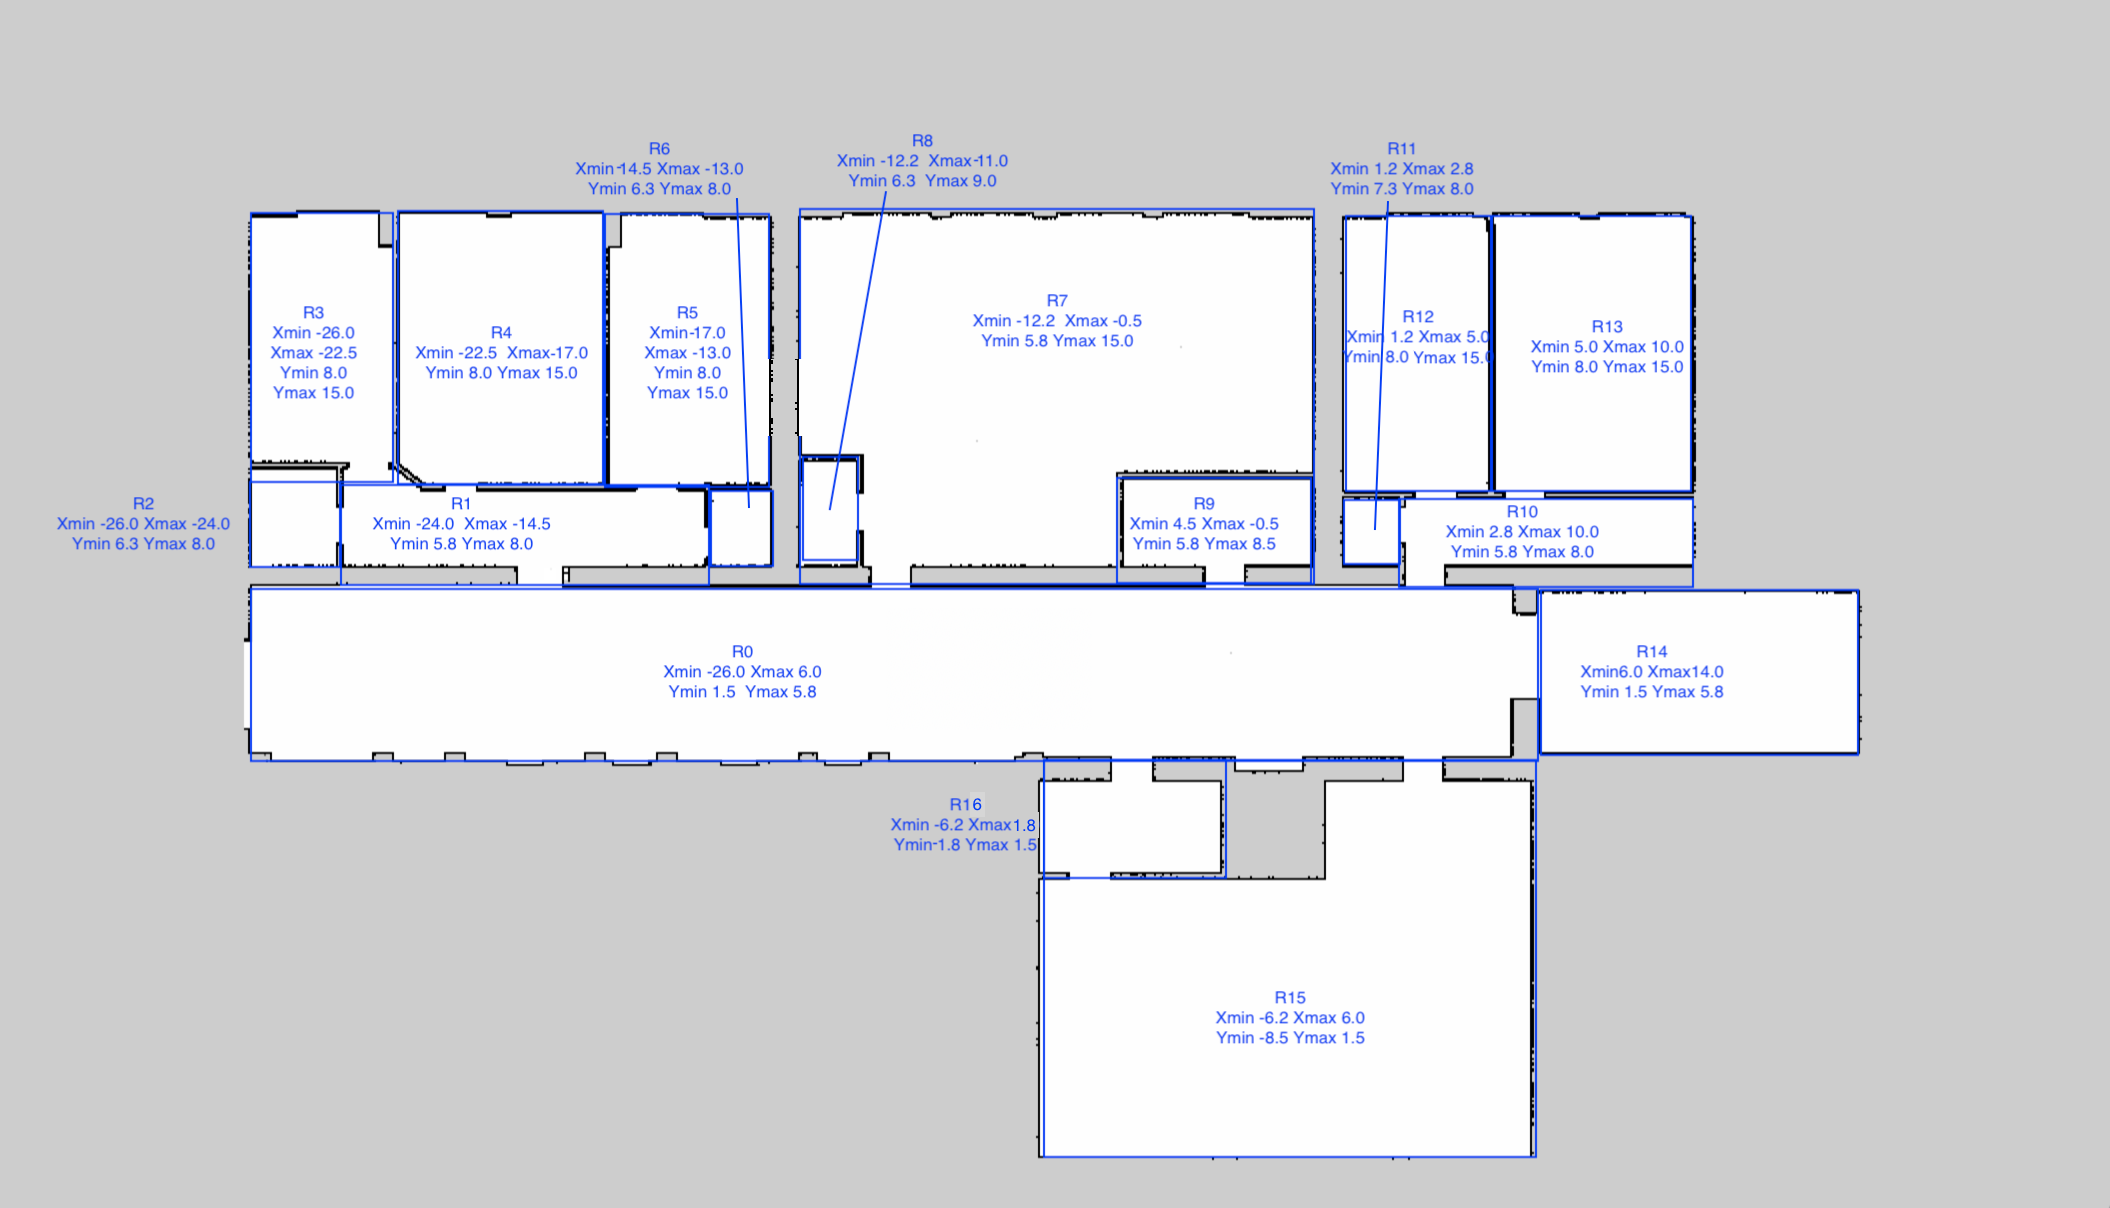
\includegraphics[width = 0.7\textwidth]{content/images/ch1/room_division.png}
 \caption{The simulated office environment. There are 16 Rooms in this office environment.}
 \label{fig:experiment_rooms}
\end{figure}

\begin{figure}
 \centering
 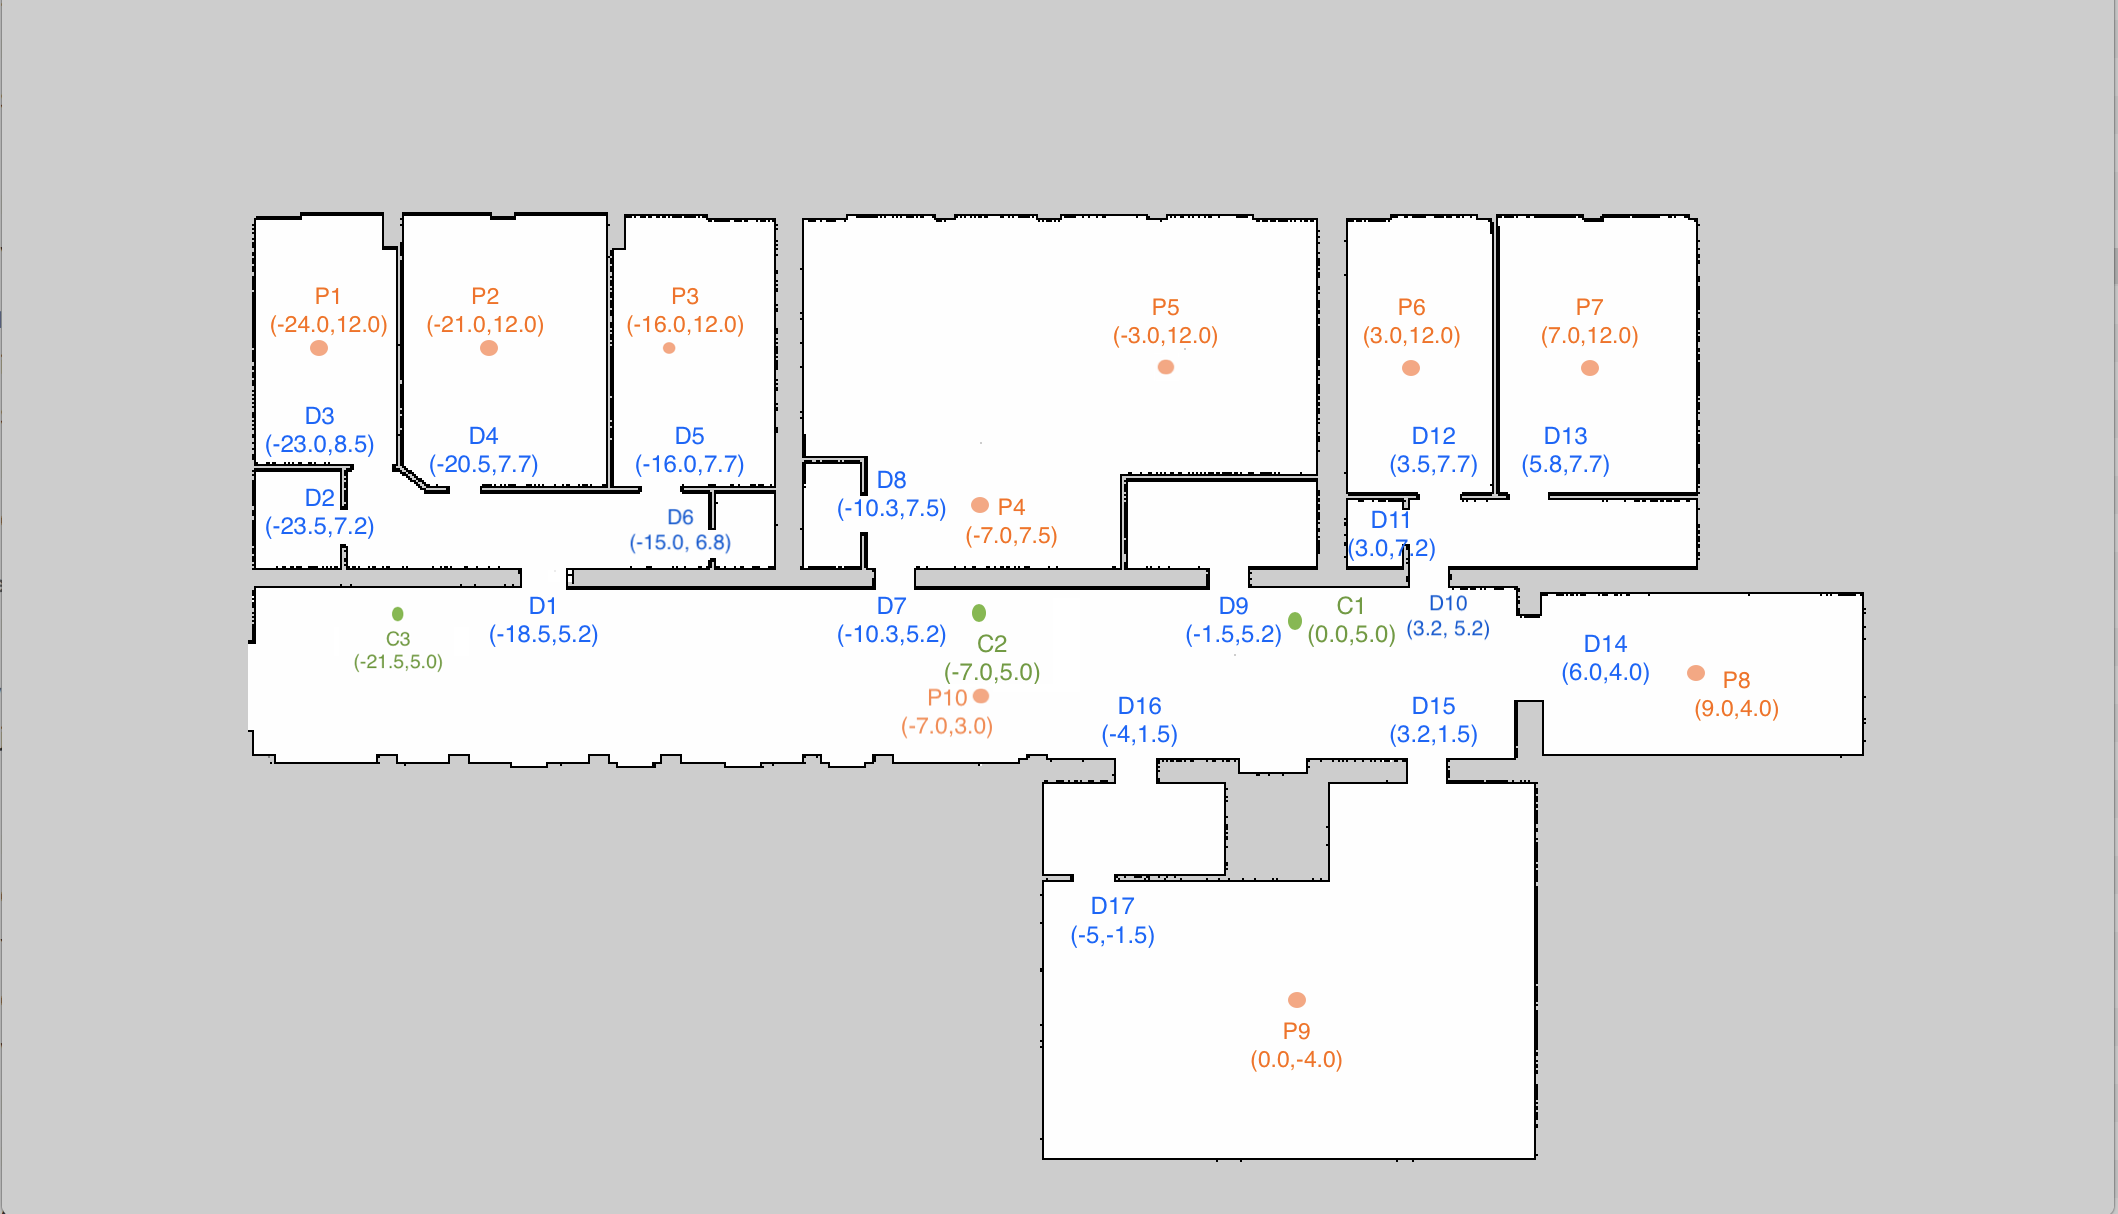
\includegraphics[width = 0.8\textwidth]{content/images/ch5/door_station_points.png}
 \caption{The position of doors and charging stations. C1-C3 are charging stations and D1-D17 are doors. The sensor attached to the door has the same position with the door. P1-P10 are target positions used in navigation experiments}
 \label{fig:door_station}
 \end{figure}

\subsection{Office Environment Simulation}
\label{sec:office_simulation}

\begin{figure}
  \centering
  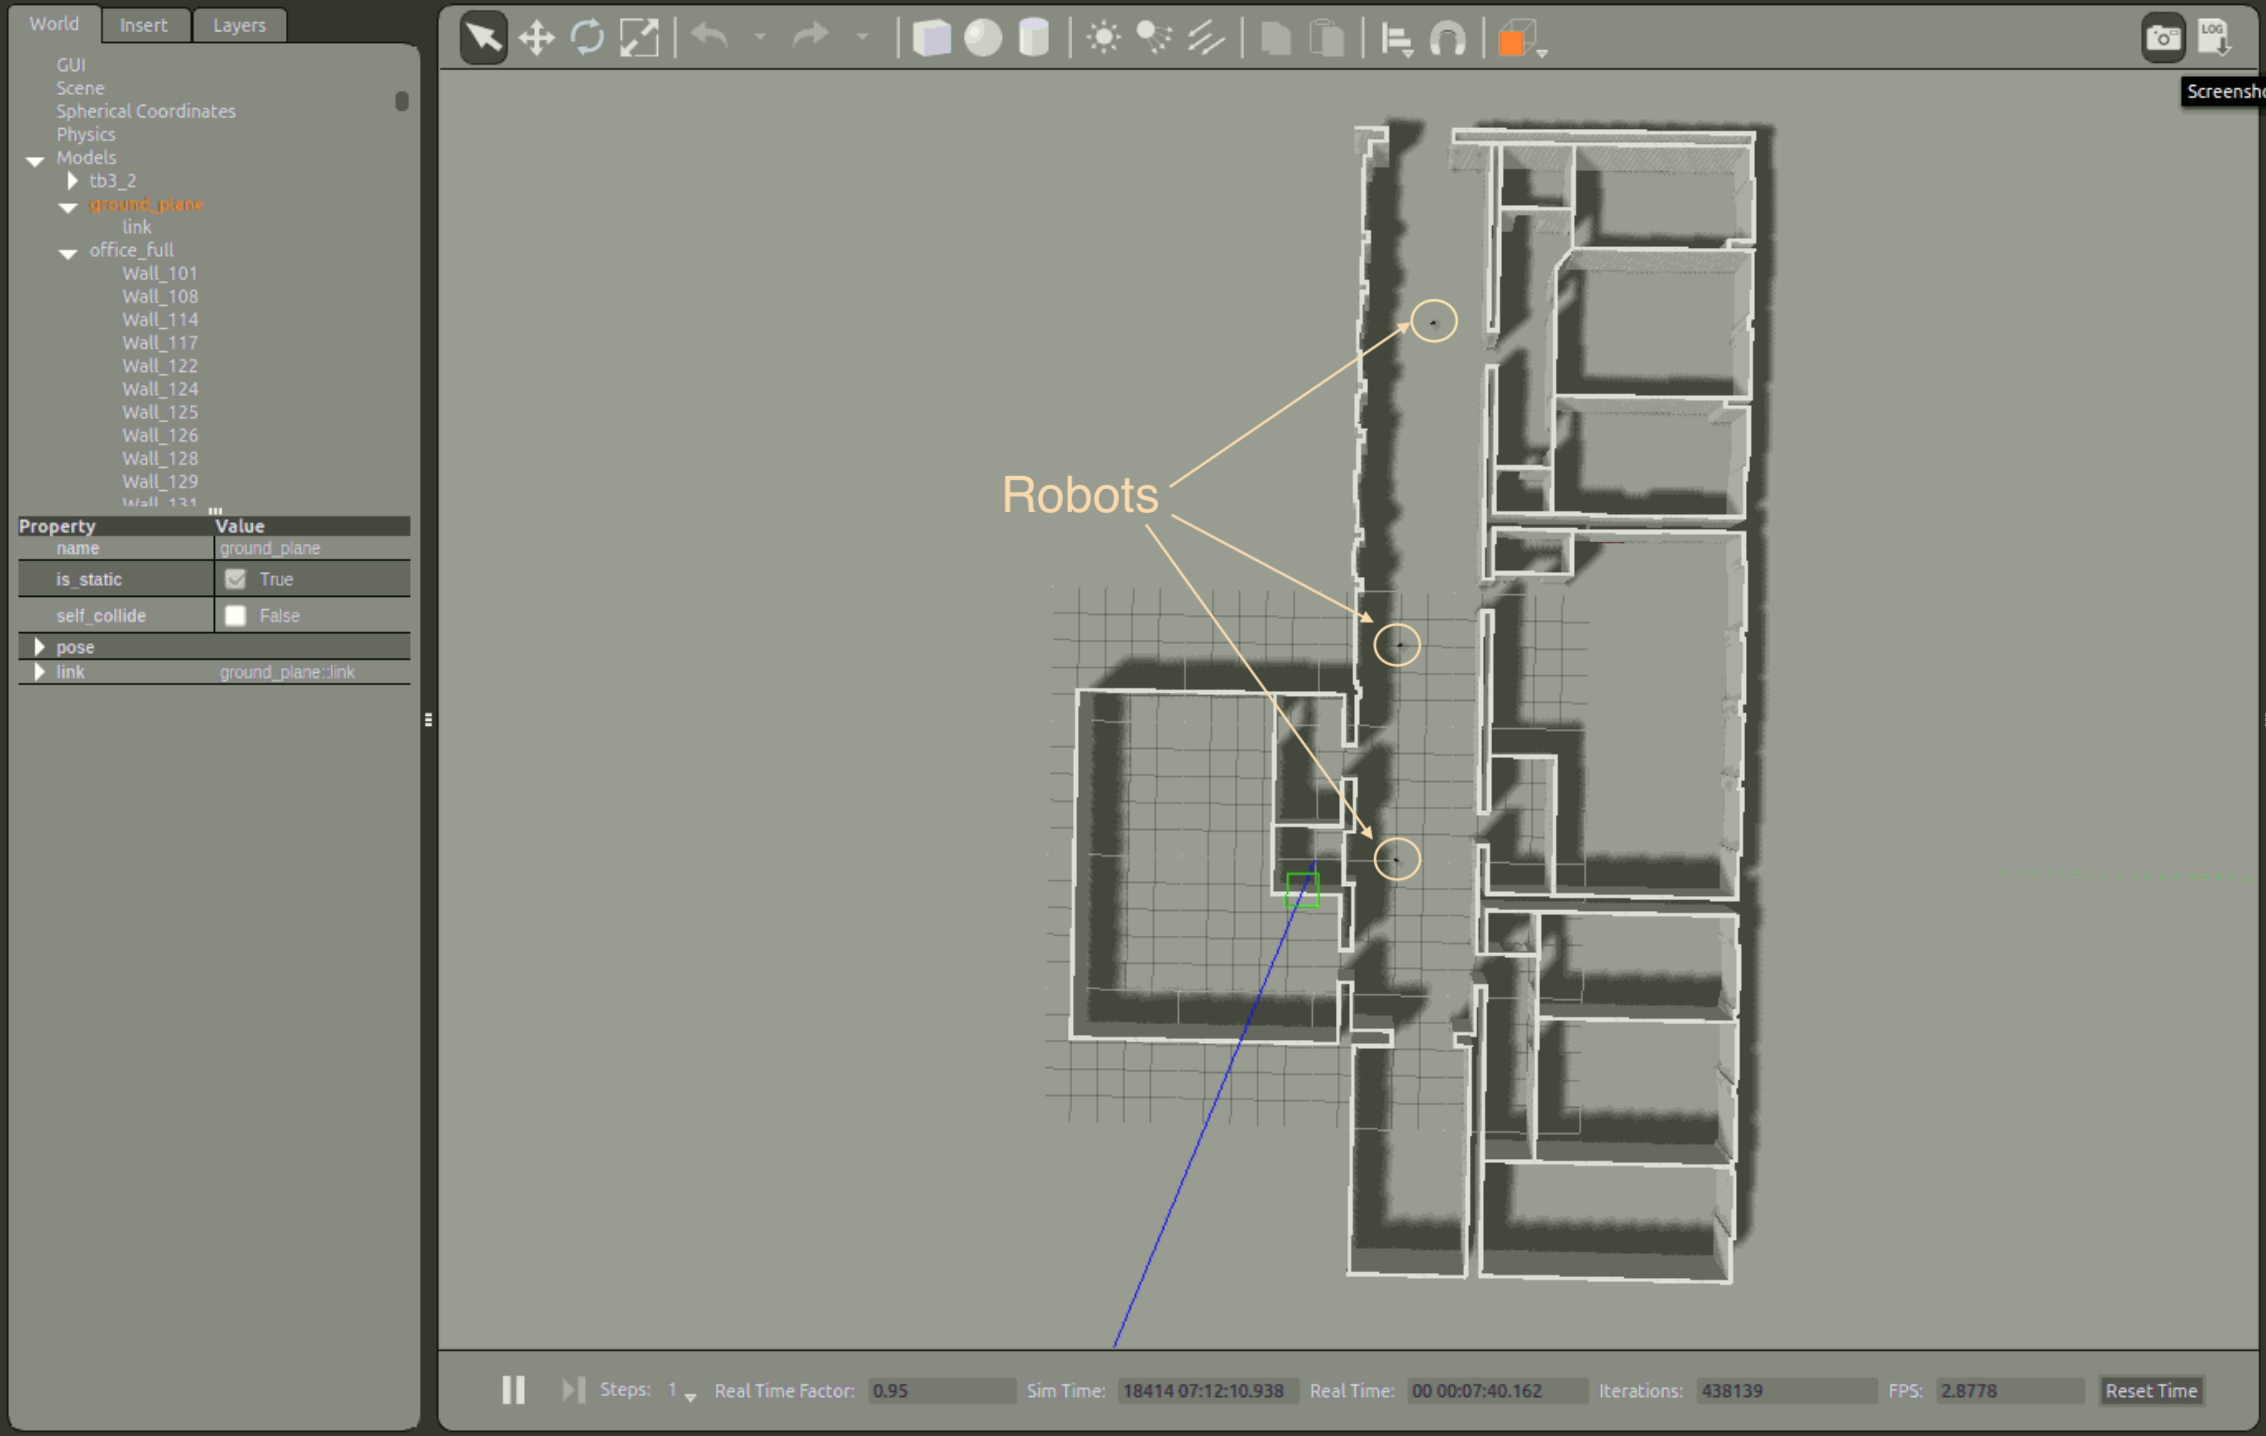
\includegraphics[width = 0.7\textwidth]{content/images/ch5/gazebo_gui_environment.png}
  \caption{The simulated office environment in Gazebo.}
  \label{fig:gazebo_simulated_office}
\end{figure}

An office environment was used to evaluate the multi-robot system. This office environment contains a corridor along the central x-axis and 16 rooms located around the corridor (Figure \ref{fig:gazebo_simulated_office}). Each room was assumed to have one or multiple doors, and each door was attached to a sensor. The sensor simulator (Chapter \ref{sec:sensor_simulation}) was used to broadcasted sensor messages periodically. There were no dynamic obstacles in this environment.

Simulation time was used in this office environment in Gazebo. All experiments used the default simulation time. The simulation time flowed fluctuates, and its flow rate was about 10\%-20\% slower than in real-time. The start and pause bottom of the Gazebo GUI interface can speed up the flow of simulation time. But speeding up by five times would cause Gazebo to crash.

\paragraph{Limitations of the office environment.} As shown in Figure 
\ref{fig:experiment_rooms}, even though the simulated working environment was very similar to the real working environment, there was one limitation: There was no door installed at the exit in the simulated working environment. As a result, even if the instant measuring data was ``door closed'', the robot can enter the rooms and successfully finish the task. However, this task needed to be canceled or done again because a door was closed. This limitation affected the number of successful tasks. 

\section{Experiment Procedure}
Two kinds of experiments were designed: gathering information experiments and navigation experiments. Charging was required between any two experiments to conduct multiple experiments one after another. In other words, at the beginning of each experiment, all robots started from their initial position, which was the charging station. After each experiment, the robot returned to the charging station to charge. For example, robot 1 charged at charging station 1, robot 2 charged at charging station 2, robot 3 charged at charging station 3. In this case, the robot would not stop moving due to a lack of energy during the experiment. 


\subsection{Gather Information Experiment}
After the simulation starts, it went to the charging station to charge. When all robots were charged, the first experiment began. In each gather information experiment, robots need to complete navigation tasks continuously. Twenty simulated minutes later, the robot first completed the current task and then returned to the charging station. The task completion status and measurement results in these 20 simulated minutes will be statistically analyzed. When all robots were charged, the next experiment starts. This experiment process is shown in \ref{fig:env_exp_timeline}.

 \begin{figure}
 \centering
 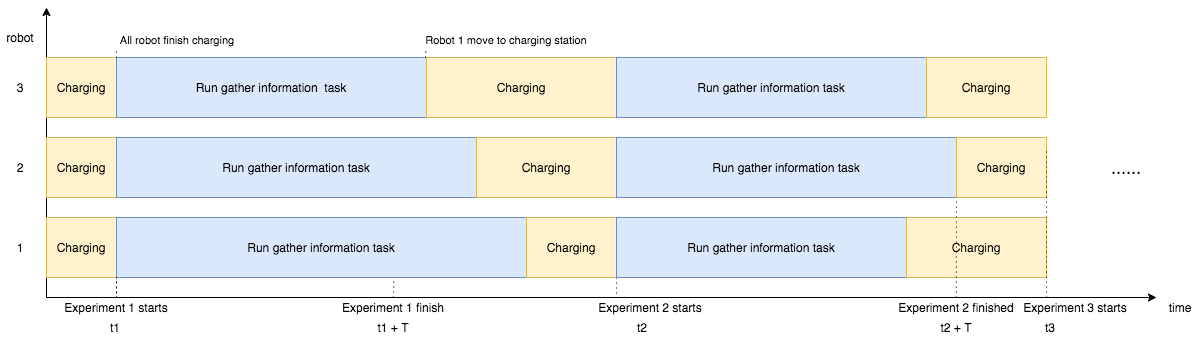
\includegraphics[width = 0.9\textwidth]{content/images/ch5/env_exp_timeline.drawio.png}
 \caption{The procedure of gather information experiment.  In each gather information experiment, robots need to complete navigation tasks continuously for 20 simulated minutes.}
 \label{fig:env_exp_timeline}
 \end{figure}


\begin{table}
\resizebox{\textwidth}{!}{
\begin{tabular}{|l|l|l|l|l|l|l|}
\hline
$W_{\mbox{energy}}$ & $W_{\mbox{last update}}$ & $W_{\mbox{probability}}$ & Average Last update Time & Average Update Interval & Succeeded Task & Failed \\ \hline
15.00   & -0.10      & -0.20   & 00:13:18     & 00:01:29      & 52        & 0      \\ \hline
15.00   & -0.10      & -0.20   & 00:14:30     & 00:01:33      & 47        & 0      \\ \hline
15.00   & -0.10      & -0.20   & 00:12:52     & 00:01:36      & 49        & 0      \\ \hline
\end{tabular}}
\caption{Example result of gather information experiment. The values of the first three columns (weight parameters) were set before the simulation experiment was started, and the values of other columns were filled after the simulation experiment.}
\label{tab:gather_infomation_experiment_result}
\end{table}

The task scheduling approach (Chapter \ref{sec:task_scheduling_approach}) make decisions base on information about robots and the environment. In this decision-making process, it was necessary to calculate the cost of robot computing tasks. At the beginning of each experiment, the weight of the cost function parameters would be changed according to the experiment result table (Table \ref{tab:gather_infomation_experiment_result}). The followings are columns of the Table:

The ``Average last update time'' factor was the time difference between experiment start time and minimal value in ``Last update'' column in the door table (Table \ref{tab:db_doors}) when an experiment finished. For example, ``Last update'' factor in experiment 1 (Figure \ref{fig:gather_info_experiment_enumerate}) was``00:02:57''. It means that the door in the worst case not be measured since 2 minutes 57 seconds (simulated time) after the experiment starts. The ``Average update interval'' means the average interval of door update. For example, ``Average Update Interval'' factor in experiment 1 (Figure \ref{fig:gather_info_experiment_enumerate}) was ``00:01:00''. It means that, on average, every door was updated every minute. The ``Succeeded Task'' factor means the number of succeeded ``gather information'' task. The ``Failed Task'' factor means the number of failed ``gather information'' task.



\paragraph{Experiment: Use Enumeration Method to Find the Best Weight Combinations}
\label{sec:gather_info_experiment_enumerate}
\subparagraph{Experiment Introduction} 
To find the best weight combinations, 30 experiment are created with $W_{\mbox{energy consumption}} \in \{ 0,1,5,10 \}, W_{\mbox{update}} \in \{-10,-5,-1\}, W_{\mbox{probability}} \in \{-10,-5,-1,0\}$. In addition, the conditions $W_{\mbox{update}}=0$ was not testable, because during the experiment centralized pool generate the same ``gather information tasks``, which let robots not moving and measuring their nearest door. Experiment Duration T = 10 min.

\paragraph{Experiment Result} 
Figure \ref{fig:gather_info_experiment_enumerate} represent the experiment result.

\begin{figure}
 \centering
 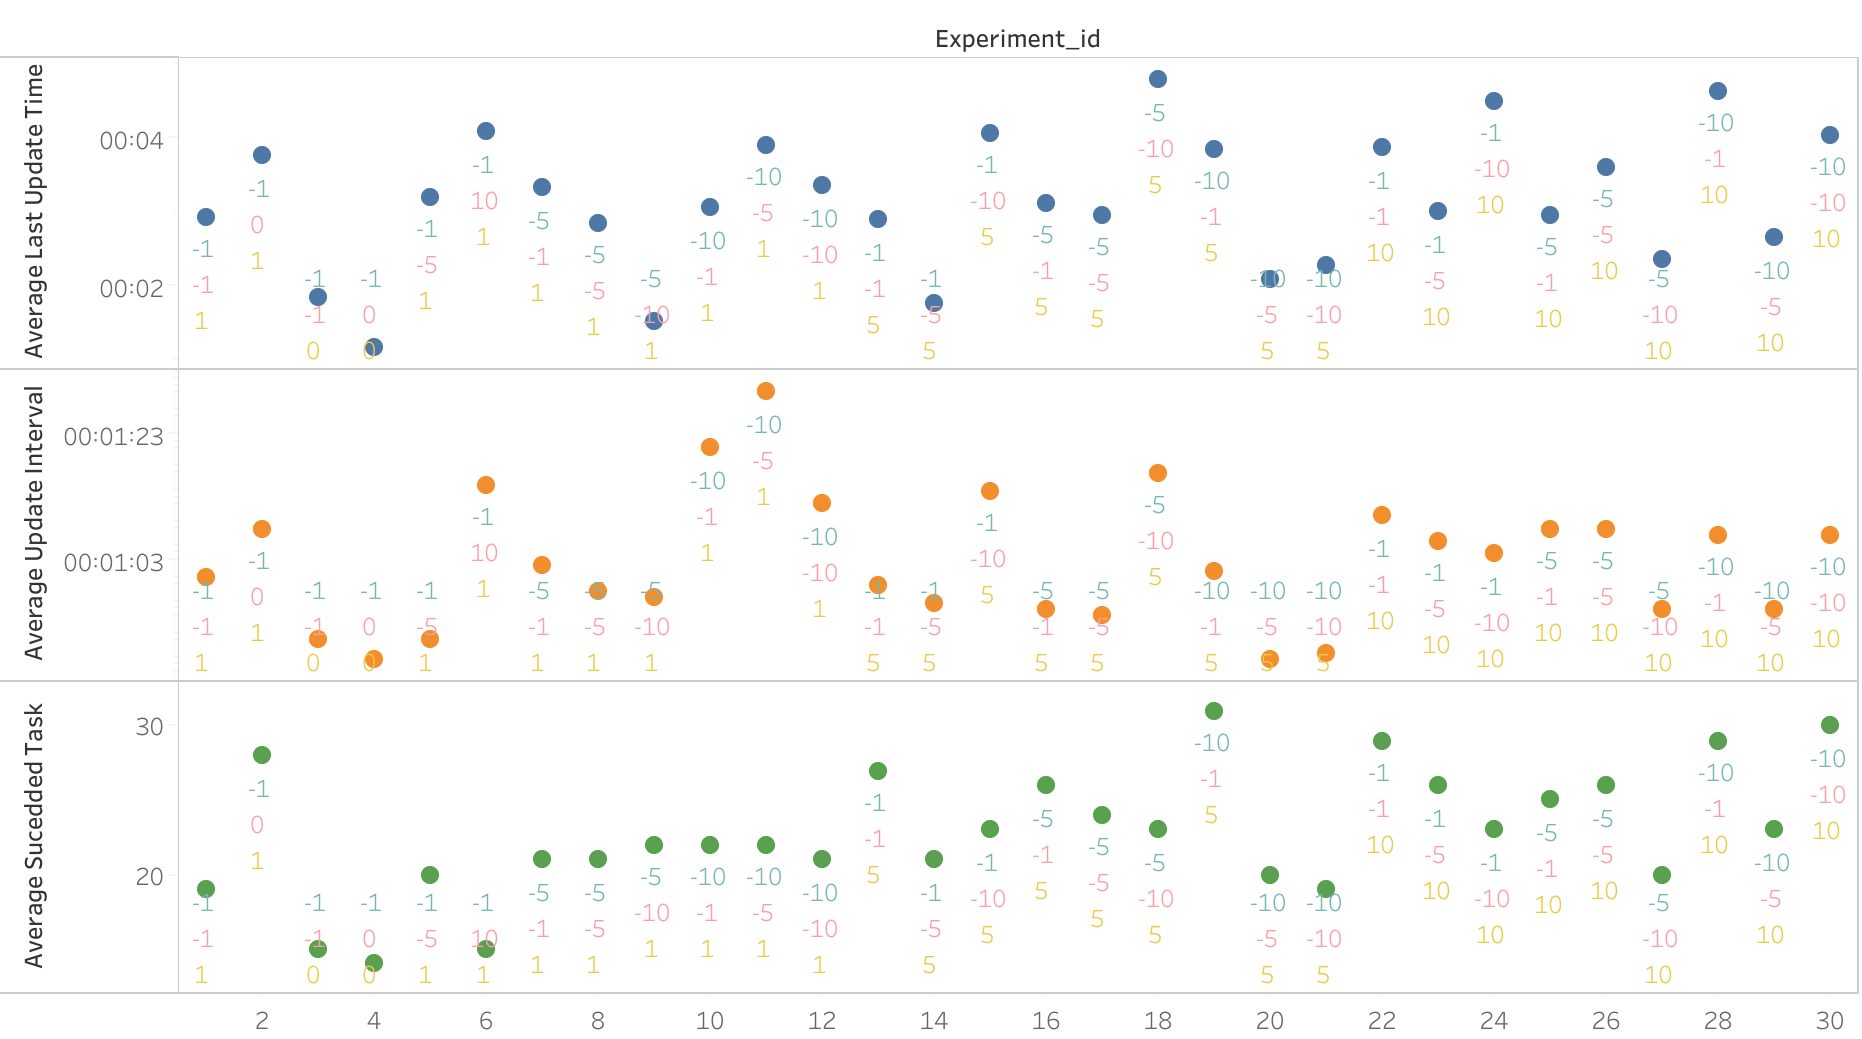
\includegraphics[width = 0.9\textwidth]{content/images/ch5/gather_info_enumerate.png}
 \caption{Use enumeration method to find best weight combination. The marks are labeled by weight combinations (energy, last update, probability).}
 \label{fig:gather_info_experiment_enumerate}
\end{figure}

\paragraph{Experiment Analysis} 


As shown in the experiment result, all ``Minimal Last Update'' value was from 1 min to 5 min, much less than the experiment duration (10 min). This shows that some rooms have very backward data. One possible reason was that the velocity of the robot was small (about 0.2 per second). The experiment duration (10min) was not long enough to let three robots pass to all doors. Another possible reason was that the robot's route was partially duplicated. For example, when the system started, robot 1 was at charging station 1 and got a task to door 3, while robot 2 was at charging station 2 and got a task to door 4. As shown in Figure \ref{fig:door_station}, these two route are partially duplicated, both of them pass through door 1 and entered room 1 (Figure \ref{fig:experiment_rooms}). The ideal solution was to give both tasks to one robot. 



\paragraph{Experiment: Use Analysis to Find the Best Weight Combinations}

\begin{figure}
 \centering
 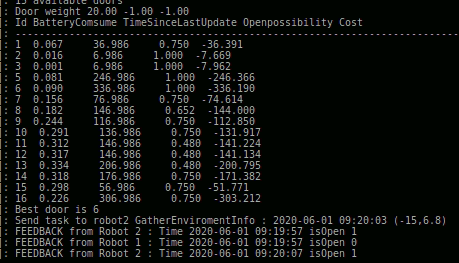
\includegraphics[width = 0.7\textwidth]{content/images/ch5/weight_analyze.png}
 \caption{The cost table in the centralized pool.}
 \label{fig:cost_table}
\end{figure}

\paragraph{Experiment Introduction} 
As is discussed in the last experiment (Chapter \ref{sec:gather_info_experiment_enumerate}), the experiment time was too short to allow the robot to explore each door. Therefore, the experiment duration in this experiment was increased to 20 min.
Firstly, we should find the best weight combination for ``weight battery'' and ``weight last update'', then find the third weight ``weight probability''. Finally, the best combination of weight will be concluded.
 According to the cost table (Figure \ref{fig:cost_table}), the update time value has a minimal value of 6.986 and a maximal value of 336.986 (column 3), which are much larger than energy consumption (column 2 in Figure \ref{fig:cost_table}) and product of door open possibilities (column 4 in Figure \ref{fig:cost_table}).
 Therefore, 18 experiments are created with $W_{\mbox{battery}}$
 = 0.1 and $W_{\mbox{battery}} \in \{1,5,10,15,20,25 \}$.


\paragraph{Experiment Result} The experiment results are shown in Figure \ref{fig:gather_info_experiment_two_value} and Figure \ref{fig:gather_info_experiment_three_value}
\begin{figure}
 \centering
 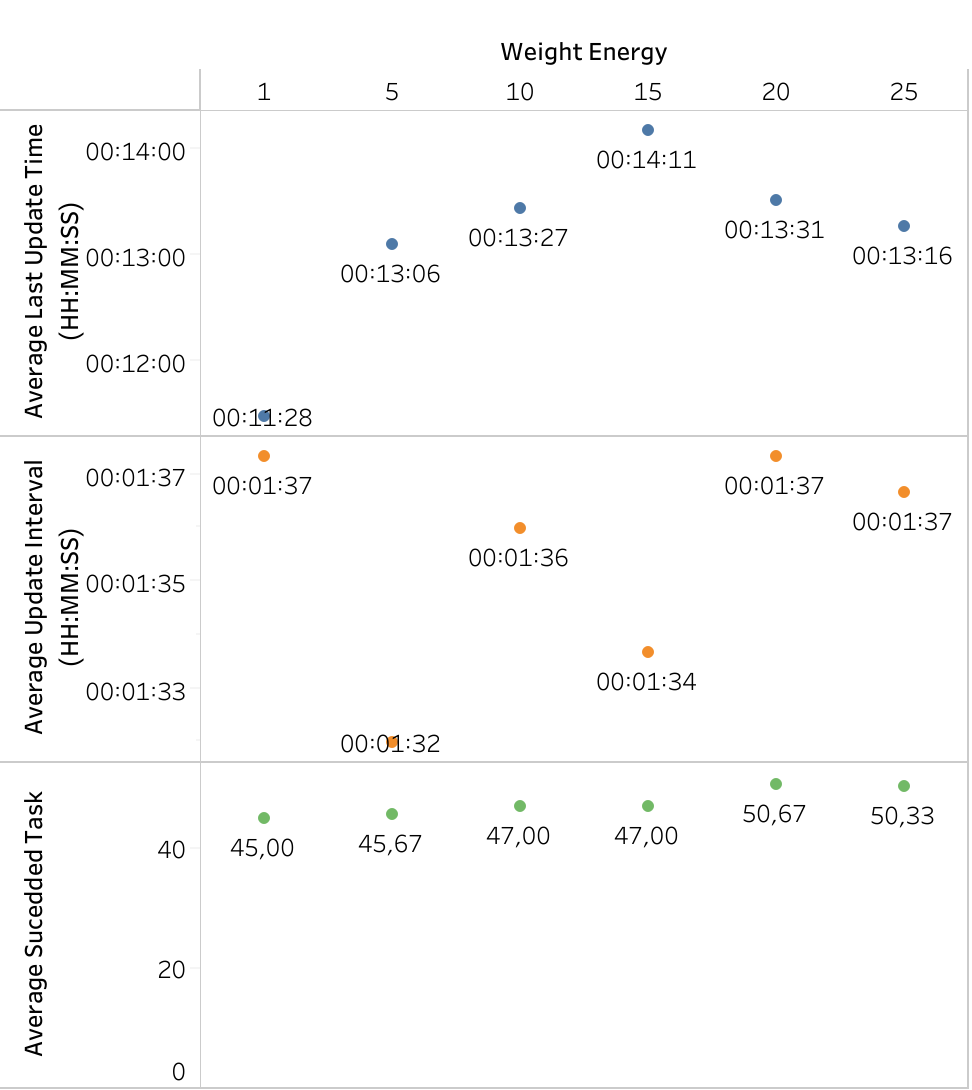
\includegraphics[width = 0.6\textwidth]{content/images/ch5/gather_info_change_weight_energy_only.png}
 \caption{Change $W_{\mbox{battery}}$ under condition $W_{\mbox{update}} = 0.1$ and $W_{\mbox{probability}}=0$}
 \label{fig:gather_info_experiment_two_value}
\end{figure}

\begin{figure}
 \centering
 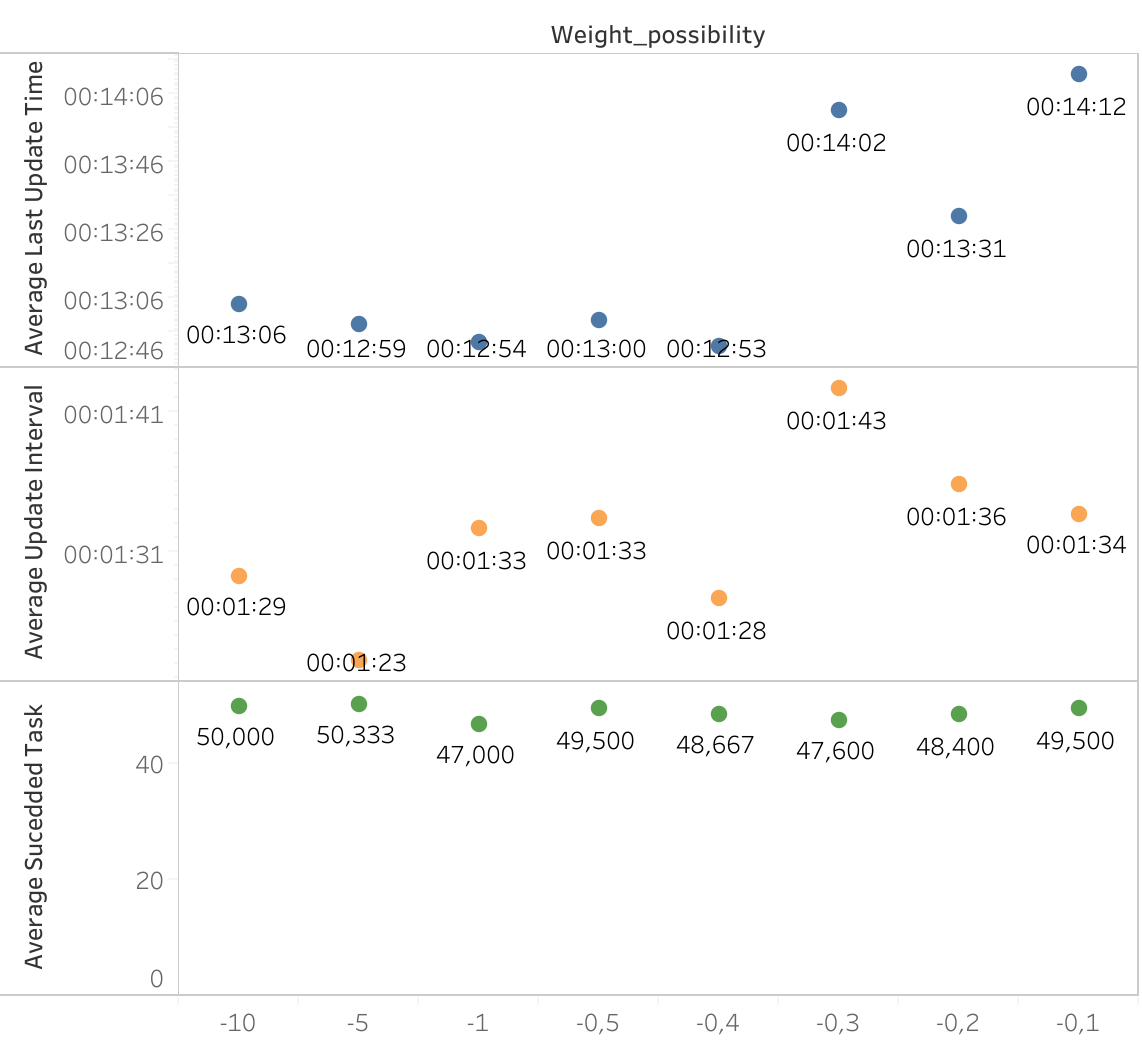
\includegraphics[width = 0.6\textwidth]{content/images/ch5/gather_info_change_weight_probability_only.png}
 \caption{Change $W_{\mbox{probability}}$ under condition $W_{\mbox{battery}}=15$ and $ W_{\mbox{update}}=0.1$}
 \label{fig:gather_info_experiment_three_value}
\end{figure}

\paragraph{Experiment Analysis} 
As shown in experiment result Figure \ref{fig:gather_info_experiment_two_value}, ``weight battery'' increased from 0 to 25, the ``average succeeded experiment task number'' slightly increased from 45 to 50, but ``average update interval'' were floated in a small range around ``00:01:35''. Especially, as ``weight battery'' increased from 0 to 15, ``average last update'' showed an upward trend, and as ``weight battery'' increased from 15 to 25, ``average last update'' showed a downward trend, 
therefore ``weight battery'' 15 and ``weight update'' 0.1 was the best combination. 
This combination was used in next experiment set (Figure \ref{fig:gather_info_experiment_three_value}). From this experiment set, it was concluded that ``weight battery'' 15, ``weight update'' 0.1, ``weight probability'' 0.1 and ``weight battery'' 15, ``weight update'' 0.1, ``weight probability'' -0.3 were two best weight combinations for the cost function. With the best weight combination, the system is able to receive the newest measuring data from all rooms. The task scheduling approach can efficiently improve the information gathering.



\subsection{Navigation Experiment}

\begin{figure}
\centering
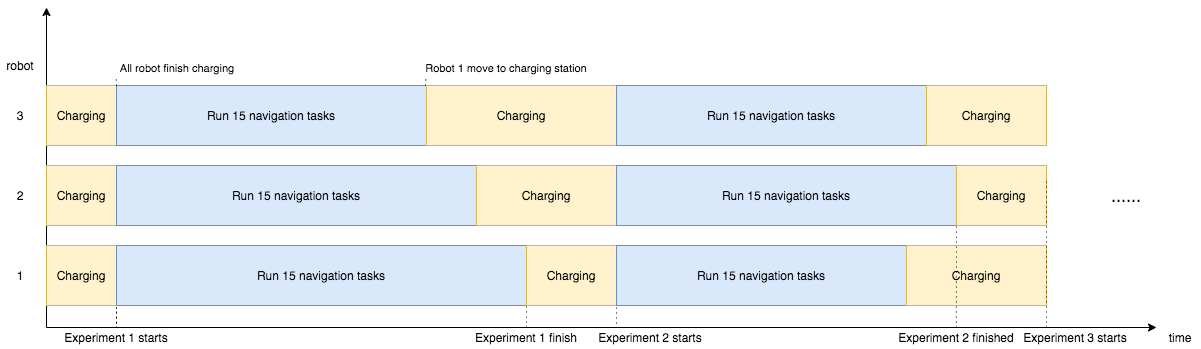
\includegraphics[width = 0.7\textwidth]{content/images/ch5/exe_exp_timeline.drawio.png}
\caption{The procedure of navigation experiments. In each experiment, 3 robots need to finish 15 navigation tasks and 3 charging tasks.}
\label{fig:nav_exp_timeline}
\end{figure}

After the simulation started, the robot went to the charging station to charge. After all the robots were charged, the first experiment began. The robot returned to the charging station to charge after completing 15 navigation tasks. The completion status and measurement results of these 15 tasks will be statistically analyzed. When all robots are charged, the next experiment starts. In other words, robots need to finish 15 navigation tasks and 3 charging tasks in each navigation experiment. The experiment start time was when all robots finished charging and started request tasks, and the experiment finish time was when the latest task was finished. This experiment process is shown in Figure  \ref{fig:nav_exp_timeline}.

The task scheduling approach (Chapter \ref{sec:task_scheduling_approach}) make decisions base on information about robots and the environment. In this decision-making process, it was necessary to calculate the cost of robot computing tasks. At the beginning of each navigation experiment, the weight of the cost function parameters would also be changed according to the experiment result table (Table \ref{tab:exp_experiment_result}). The followings are columns in the table:

The experiment duration was a critical evaluation factor in this table, which was the time difference between the experiment start time and experiment finished time. The end state of navigation tasks was evaluated. In an experiment result table, the ``Succeeded Task'' column counted the tasks ended with the succeeded state, the ``Expired Task'' column counted the tasks ended with the created state, the ``Failed'' column counted the tasks ended with states including running, error or canceled states. 

\begin{table}
\centering
\resizebox{\textwidth}{!}{
\begin{tabular}{|c|c|c|c|c|c|c|c|c|c|c|c|} 
\hline
Experiment & $W_{\mbox{battery}}$ & $W_{\mbox{waiting time}}$ & $W_{\mbox{door open probability}}$ & $W_{\mbox{priority}}$ & Experiment Duration &Total Task & Succeeded Task & Expired Task & Failed Task \\
\hline
1 & 1.00 & 1.00 & -1.00& -1.00& 00:18:23 & 15 & 15 & 0 & 0 \\\hline
2 & 1.00 & 0.00 & 0.00 & 0.00 & 00:17:23 & 15 & 7 & 8 & 0 \\ \hline
3 & 0.00 & 1.00 & 0.00 & 0.00 & 00:18:56 & 15 & 15 & 0 & 0 \\\hline
4 & 0.00 & 0.00 & -1.00 & 0.00 & 00:18:41 & 15 & 5 & 10 & 0 \\\hline 
5 & 0.00 & 0.00 & 0.00 & -1.00& 00:17:21 & 15 & 3 & 12 & 0 \\ \hline
\end{tabular}}
\caption{Example result of navigation experiment. The values of the first four columns (weight parameters) were set before the simulation experiment was started, and the values of other columns were filled after the simulation experiment.}
\label{tab:exp_experiment_result}
\end{table}

\paragraph{Experiment: Find the Best Weight Combinations}
\paragraph{Experiment Introduction}
The task time interval may affect experiment duration and experiment succeeded rate in addition to the cost function. Therefore, three sets of experiments are generated to find the best weight combinations. 

\paragraph{Experiment Result} 
Figures \ref{fig:experiment_task_30s}, \ref{fig:experiment_task_45s} and \ref{fig:experiment_task_65s} show experiment results when the task time interval is 30, 45 and 65 seconds separately. 
In addition, when the task time interval is 30 seconds, the task success rate is about 0.67. When the task time interval is 45 seconds, the task success rate is about 0.76. 
When the task time interval is 65 seconds, the task success rate is 1.0. The maximal and minimal value of y-axis are labeled.
\paragraph{Experiment Analysis} 
\begin{enumerate}
 \item \textbf{The relationship between task time interval and task success rate.} Firstly, it was concluded that the longer the task time interval, the higher the task success rate.
 This is because when the task time interval is longer, when the centralized pool select task to robot, there are fewer expired tasks that can not be selected in the task table. This leads to fewer expired tasks when an experiment is finished. Besides, in the simulation experiment, most task can be successfully finished, unless the robot collide with each other, which is time-consuming and cause task failure. Therefore, the fewer expired task results in a higher task success rate.
 \item \textbf{The best weight combinations.} When an experiment result has the most successful tasks and lowest experiment duration, the corresponding task combination can be seen as one of the best weight combinations. As shown in experiment result, the best weight combinations for different task time interval are different. 
 The best weight combination is labeled in Figure \ref{fig:experiment_task_30s} and Figure \ref{fig:experiment_task_45s} and listed in Table \ref{tab:best_weight_combinations}. However, the experiment result with most successful tasks and lowest experiment duration does not exist in \ref{fig:experiment_task_65s}. This may because the task time interval is too long, causing the robot to wait after a while before starting the next task after current task is finished. The experiment duration is mainly determined by the last task. Therefore, it is very likely that the experiment duration of many experiments are the same.
\begin{table}
 \centering
 \begin{tabular}{|c|c|c|c|c|c|c|c|c|c|c|c|} 
 \hline
 $W_{\mbox{battery}}$ & $W_{\mbox{waiting time}}$ & $W_{\mbox{door probability}}$ & $W_{\mbox{priority}}$ \\
 \hline
 15 & 15 & 15 & -1 \\ \hline
 1 & 1 & -30 & -1 \\ \hline
 1 & 20& -20 & -1 \\ \hline
 1 & 25& -1 & -1 \\ \hline
 5 & 1 & -5 & -5 \\ \hline
 50 & 30 & 0 & 0 \\ \hline
 \end{tabular}
 \caption{Best weight combinations.}
 \label{tab:best_weight_combinations}
 \end{table}
\end{enumerate}

It was concluded that the longer the task time interval, the higher the task success rate.

\begin{figure}
 \centering
 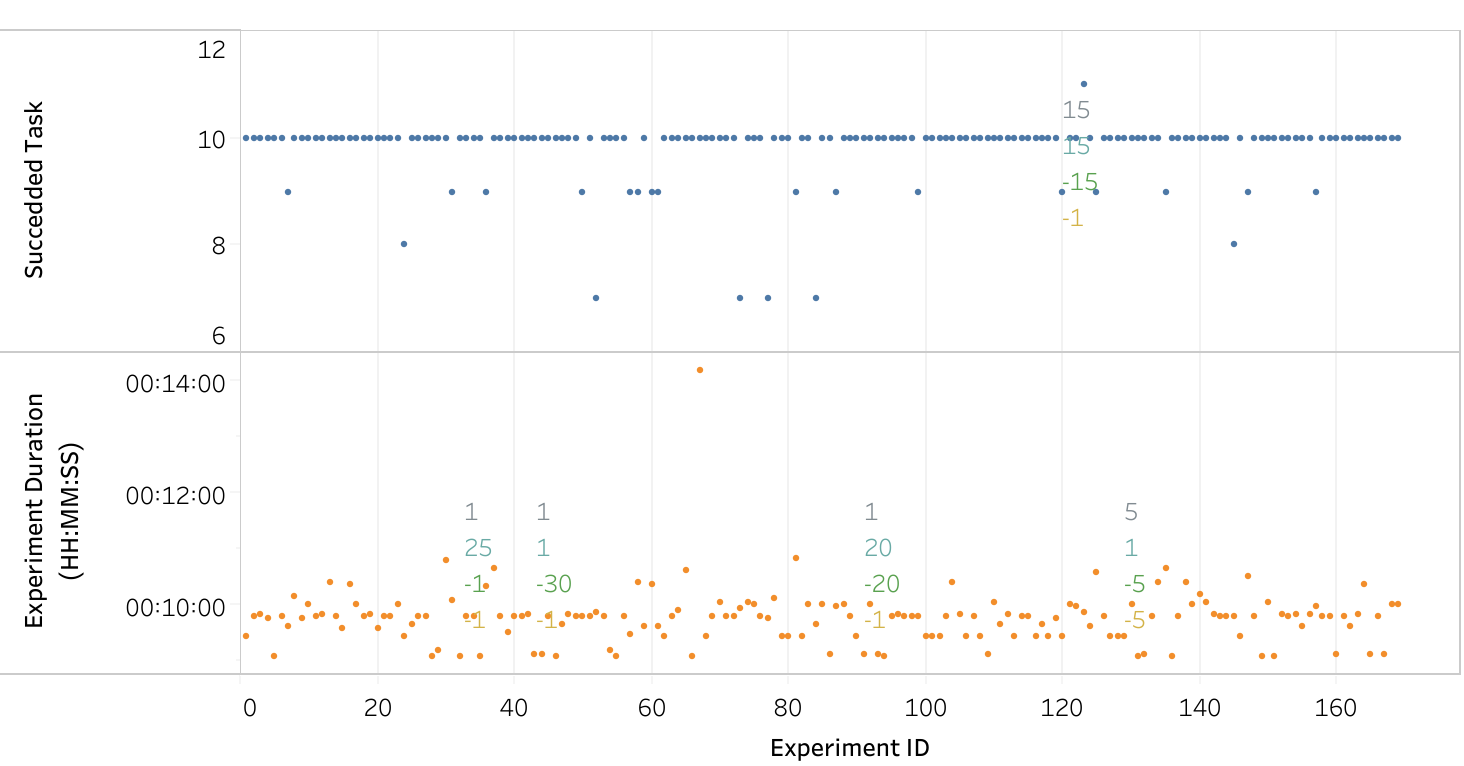
\includegraphics[width = 1.0\textwidth]{content/images/ch5/execute_experiment_30s.png}
 \caption{In each experiment, 15 ``navigation tasks'' were created with the interval of 30 seconds. The best weight combinations are labeled (energy consumption, waiting time, probability, priority).}
 \label{fig:experiment_task_30s}
\end{figure}

\begin{figure}
 \centering
 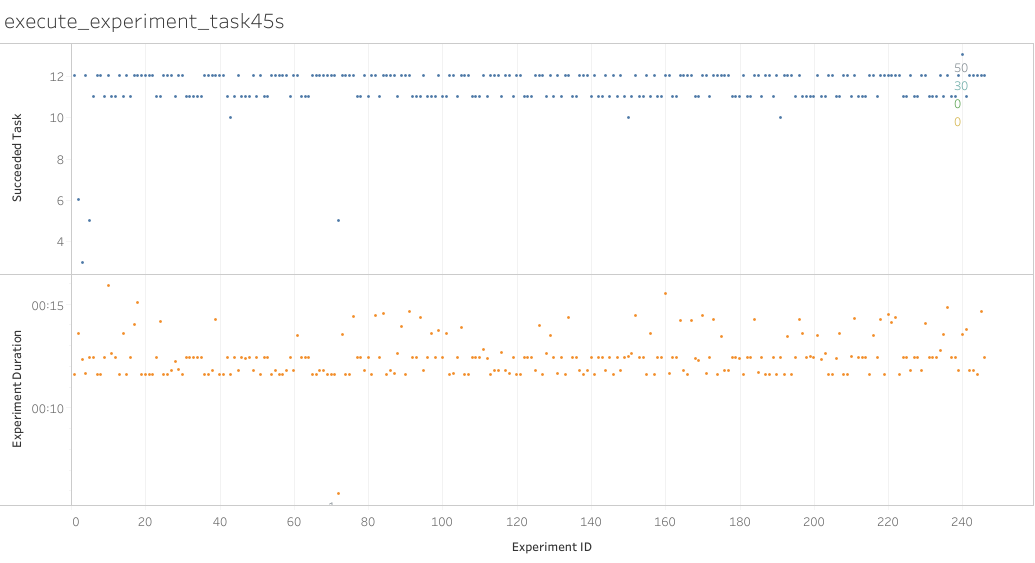
\includegraphics[width = 1.0\textwidth]{content/images/ch5/execute_experiment_45s.png}
 \caption{In each experiment, 15 ``navigation tasks'' were created with the interval of 45 seconds. The best weight combinations are labeled (energy consumption, waiting time, probability, priority).}
 \label{fig:experiment_task_45s}
\end{figure}

\begin{figure}
 \centering
 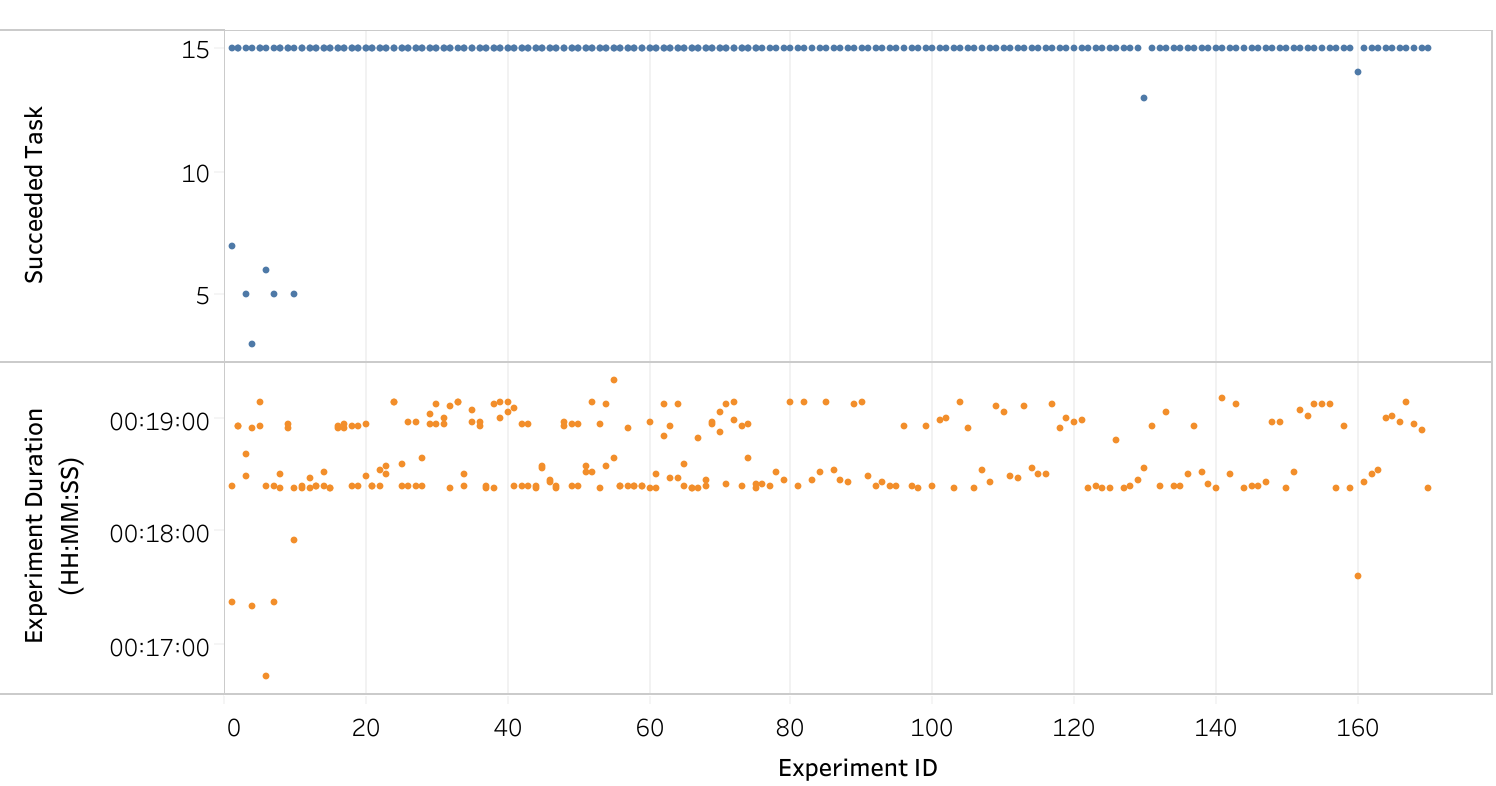
\includegraphics[width = 1.0\textwidth]{content/images/ch5/execute_experiment_65s.png}
 \caption{In each experiment, 15 ``navigation tasks'' were created with the interval of 65 seconds.}
 \label{fig:experiment_task_65s}
\end{figure}

\paragraph{Experiment: How the Number of Robots impact task scheduling}

\paragraph{Experiment Introduction} 
In this set of experiments, how the number of robots affected task scheduling was evaluated. One of the best weight combination was selected: $ W_{\mbox{battery}} = 10,W_{\mbox{waiting time}} = 1, W_{\mbox{probability}} = -1, W_{\mbox{priority}} = -10 $. 
 
\paragraph{Result} The experiment result is shown in Figure \ref{fig:different_number_of_robot}.

\paragraph{Analysis} As discussed in Chapter \ref{sec:task_scheduling_procedure}, it is concluded that as the number of robots increased, the task success rate and experiment duration increased. The reason is that the robots requested tasks from the centralized pool, respectively. The more robots there were, the more tasks could be finished in an experiment. 
On the other hand, on average, one robot could finish 7 tasks in 17 minutes and 40 seconds in simulated time, two robots could finish 11 tasks in 18 minutes and 24 seconds in simulated time, and 3 robots could finish 15 tasks in 18 minutes and 52 seconds in simulated time. It could be inferred that the more robots, the higher the efficiency of task scheduling.

\begin{figure}
 \centering
 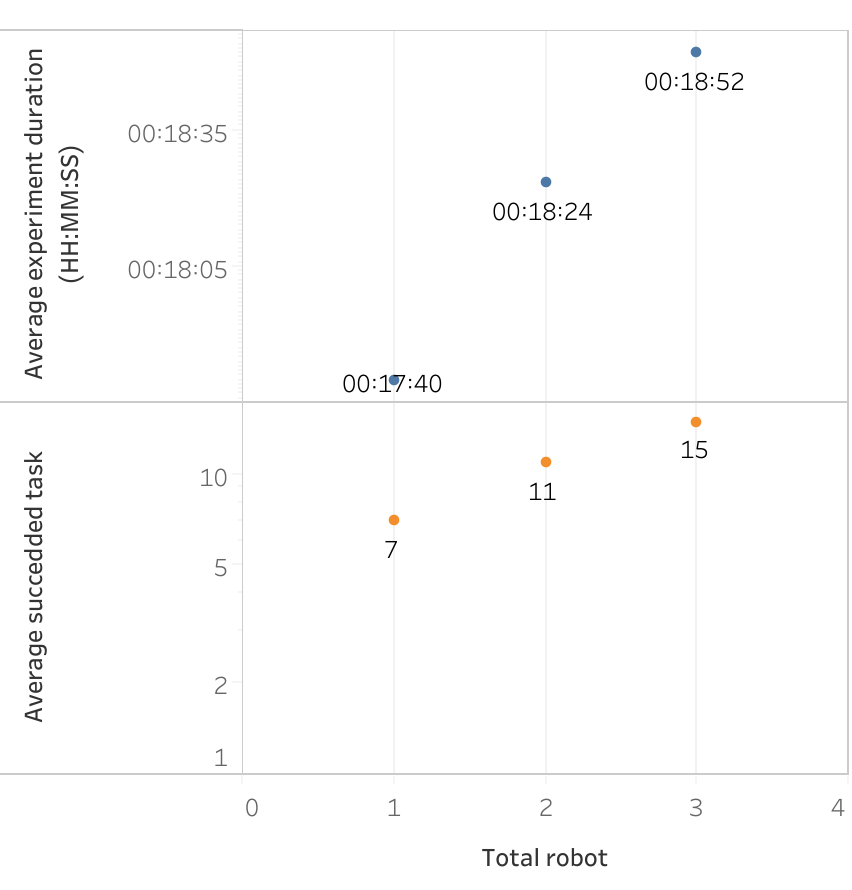
\includegraphics[width = 0.4\textwidth]{content/images/ch5/different_number_of_robots.png}
 \caption{How the number of robots impacts task scheduling}
 \label{fig:different_number_of_robot}
\end{figure}

\paragraph{Experiment: Evaluation of how my approach improves navigation tasks scheduling}

\paragraph{Experiment Introduction} 
This set of experiments evaluated how my approach \ref{sec:task_scheduling_approach} improves the scheduling of ``navigation task''. Some experiments did not use the algorithm, and others used the designed algorithm and used the best weight combination. The experiment results will be analyzed to determine how much the designed algorithm can improve task scheduling.

\paragraph{Experiment Result} 
The experiment result is shown in Figure \ref{fig:improvement_evaluation}. In the first four experiments, the algorithm was not used because only one decision variable is considered. In the last experiment, the algorithm was used with the best weight combination.
 This experimental Result shows the difference between using the algorithm and without using the algorithm. Compared with the case that only considered the task priority, the number of successful tasks significantly increased after using the algorithm. Compared with the situation that was only waiting time are considered, all tasks were finished in both situations, but the duration of the experiment decreased. 
%The experiment result (Table \ref{tab:exp_experiment_result}.) shows that in experiment 1, all 15 tasks were successfully finished with minimal experiment duration. In experiments 2, 4, 5, more than half of the tasks was expired. In experiment 3, all tasks were successfully finished, but it took more time than experiment 1. 
The experiment 6-24 (Figure \ref{fig:only_one_decision_variable_changed}) evaluated each decision variable separately.

\begin{figure}
   \centering
   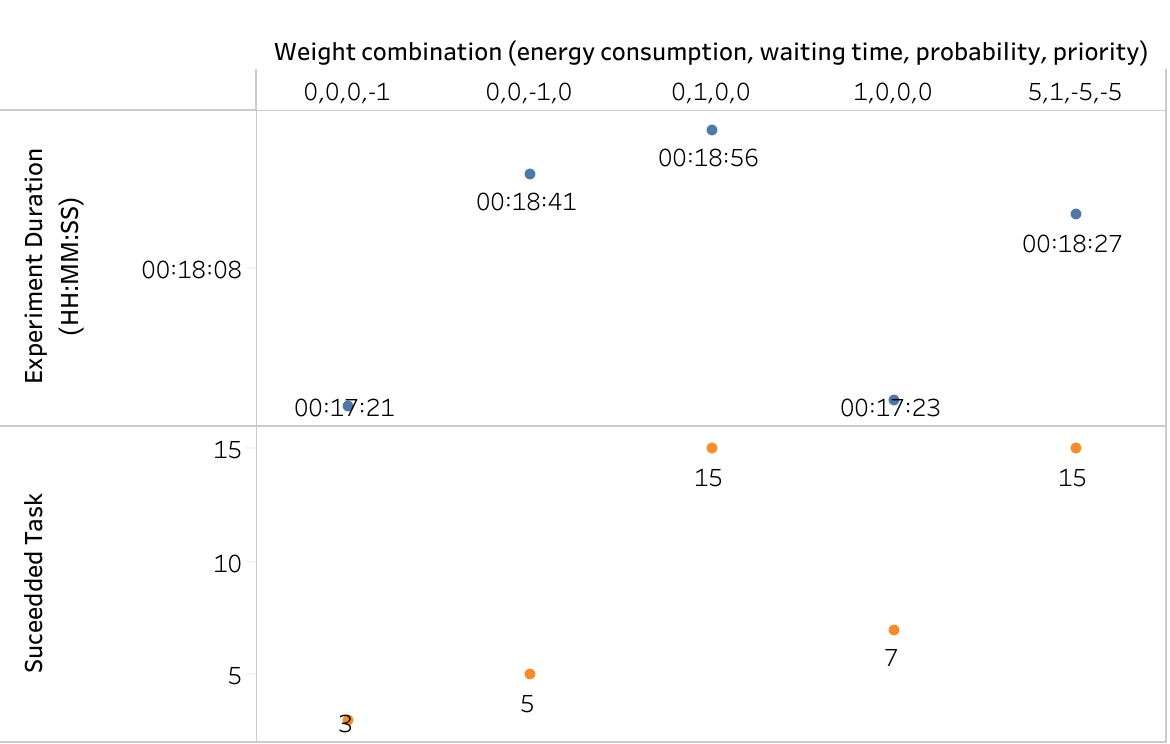
\includegraphics[width = 0.7\textwidth]{content/images/ch5/improvement_evaluation_65s.png}
   \caption{How the algorithm improves navigation task scheduling. In each experiment, 15 ``navigation tasks'' with the task interval of 65 seconds were created.}
   \label{fig:improvement_evaluation}
  \end{figure}

\begin{figure}
   \centering
   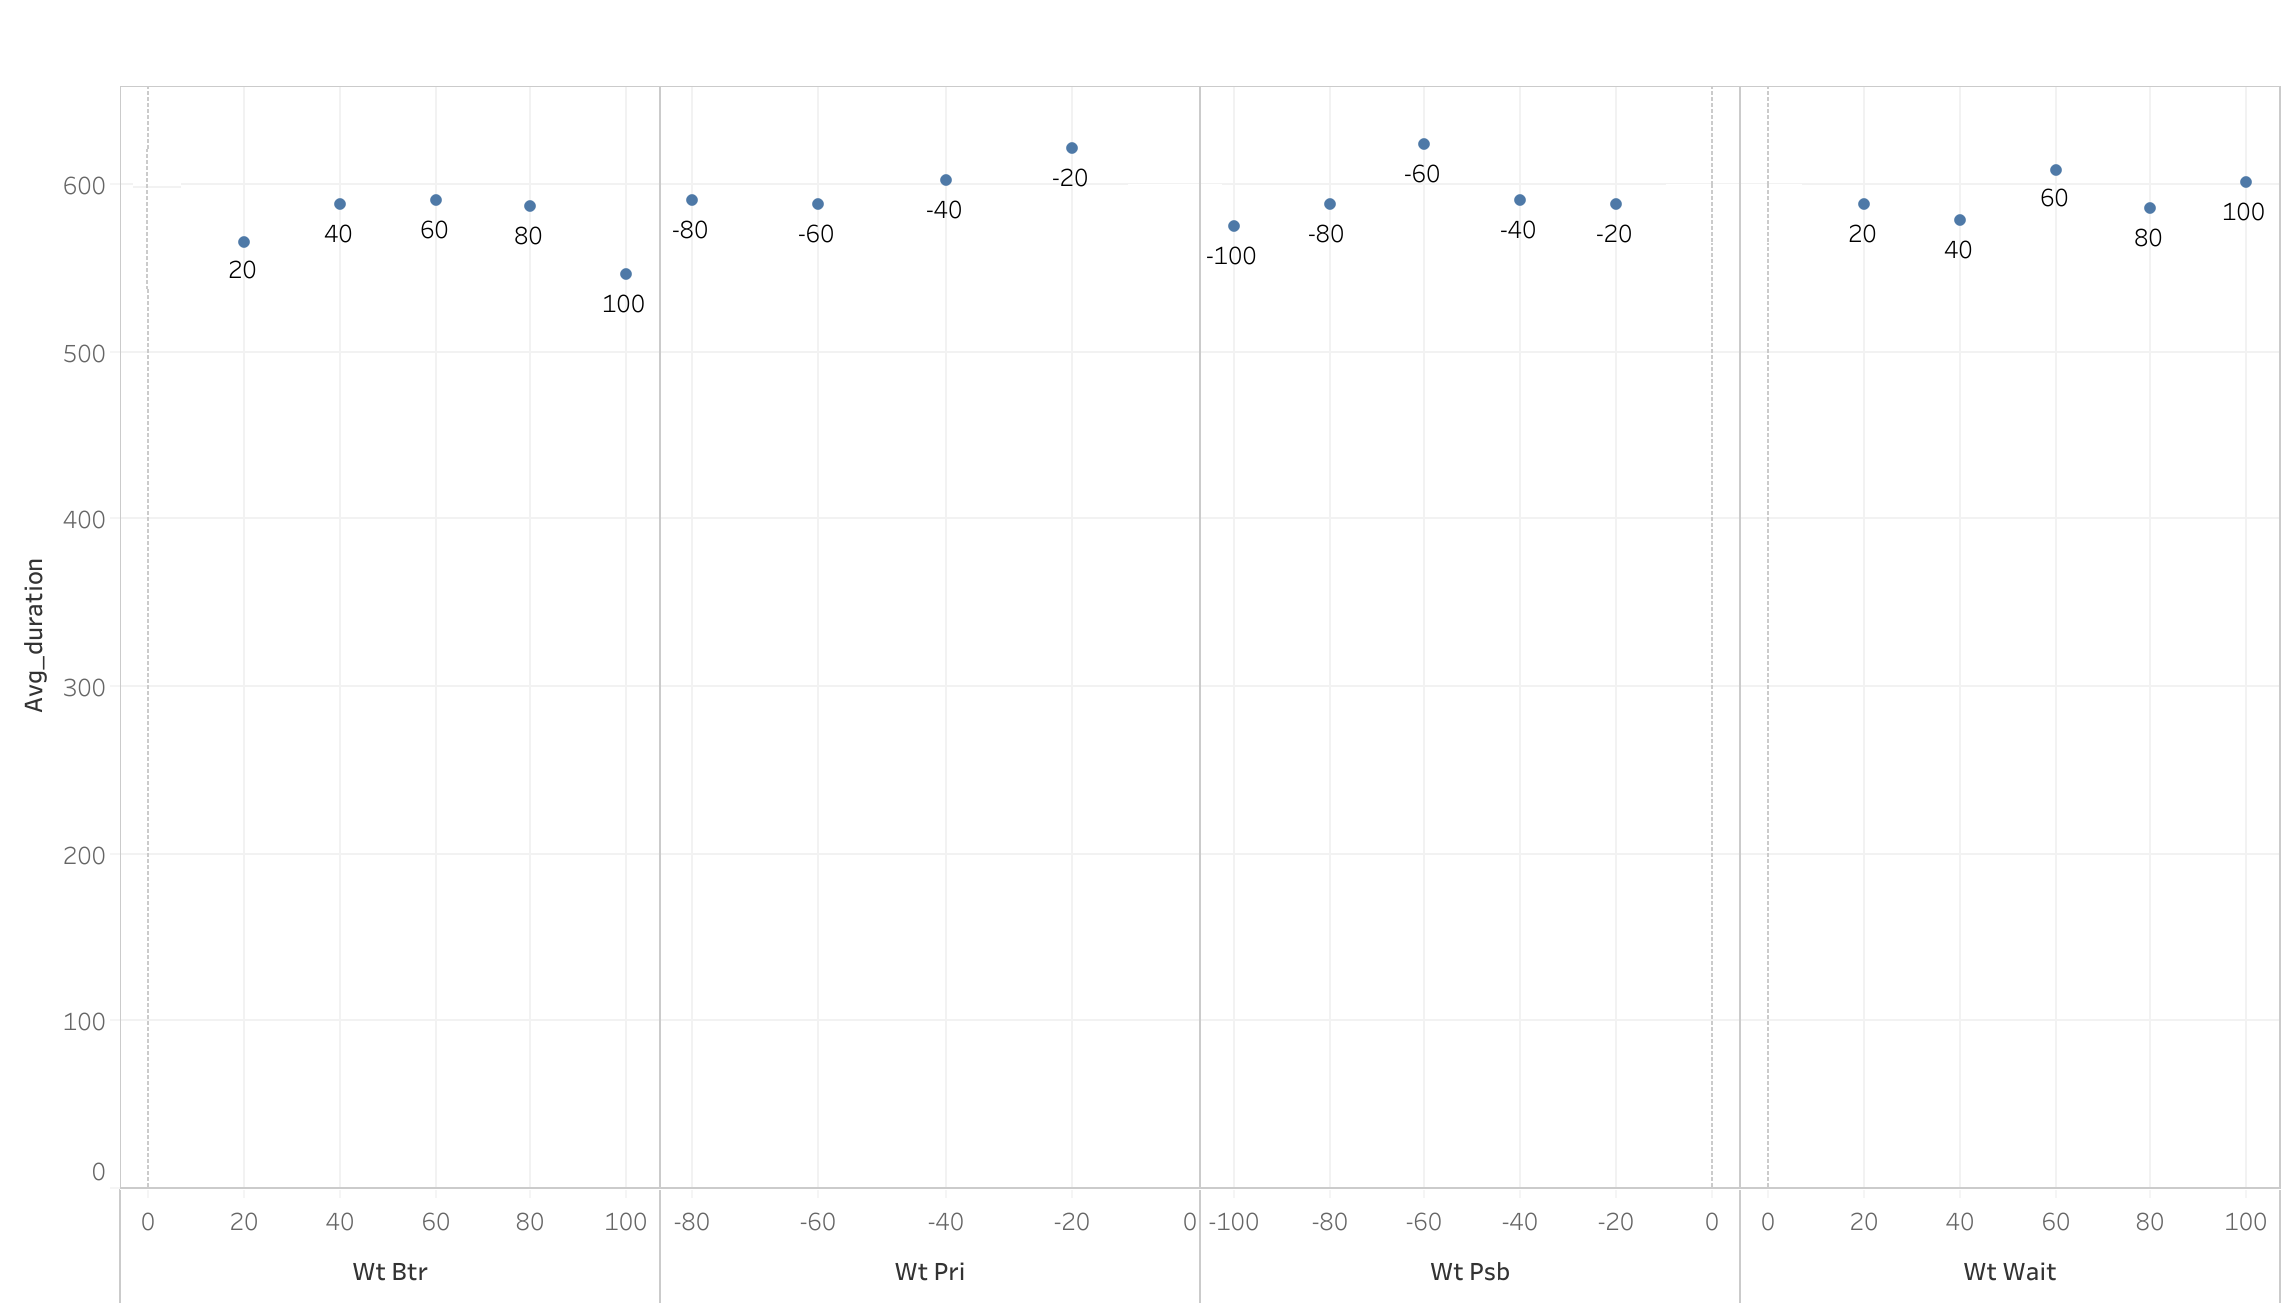
\includegraphics[width = 0.9\textwidth]{content/images/ch5/one_decision_variable.png}
   \caption{Only one decision variable changed others unchanged.}
   \label{fig:only_one_decision_variable_changed}
  \end{figure}



\paragraph{Experiment Analysis.} 
The experimental results can preliminarily judge that this algorithm has a certain effect, but this effect is not particularly obvious because the simulation experiment is limited. Following are the explanation of each decision variables:
\begin{itemize}
 \item \textbf{Door Open probability.} The door open probability is used in the algorithm to make the robot more likely to go to an occupied room. As discussed in Chapter \ref{sec:office_simulation}, the robot can enter any room, even if its door is closed. This limitation caused the room occupancy rate not to affect the number of successful tasks and the experiment duration.
 \item \textbf{Task Priority.} Similarly, the task's priority is applied by the algorithm to allow the higher priority tasks to be executed first. However, the task priority had little effect on the experiment's two evaluation criteria: the number of successful tasks and the experiment duration. If further experiments are conducted, such as evaluating the completion of high-priority tasks, then how the priority affects task scheduling can be evaluated.
 \item \textbf{Energy consumption.} The energy consumption of the robot is considered to allow low-energy tasks to be executed first. But energy consumption had little effect on the experiment's two evaluation criteria: the number of successful tasks and the experiment duration. As discussed in Chapter \ref{sec:limitations}, the energy consumption of robots in real experiments may be accurately estimated. Then further experiments can be conducted. For example, evaluating each experiment's energy consumption, then how energy consumption affects task scheduling can be evaluated.
 \item \textbf{Waiting Time.} The task's waiting time is used in the algorithm to let the earliest tasks be executed first. As shown in Figure \ref{fig:improvement_evaluation}, the waiting time significantly optimizes task scheduling. After considering this decision variable, more tasks were successfully finished, and the experiment duration was decreased. In other words, the time required to complete all tasks was reduced. Therefore, the waiting time is a crucial decision variable in the algorithm.
\end{itemize}



\begin{table}
\resizebox{\textwidth}{!}{
\begin{tabular}{|c|c|c|c|c|c|c|c|c|c|}
\hline
Task ID & Task Name & Start Time & Target ID & Robot ID &Priority & Task Status & Dependency & Finish Time & Description \\ \hline
1 & Charging & NULL & 18 & 1 & 5 & Succeeded & 0 & 2020-06-02 11:03:12 & Succeeded \\ \hline
2 & Charging & NULL & 19 & 2 & 5 & Succeeded & 0 & 2020-06-02 11:03:12 & Succeeded \\ \hline
3 & Charging & NULL & 20 & 3 & 5 & Succeeded & 0 & 2020-06-02 11:03:11 & Succeeded \\ \hline
4 & Navigation & 2020-06-02 11:04:17 & 21 & 3 & 2 & Succeeded & 0 & 2020-06-02 11:05:16 & Succeeded \\ \hline
5 & Navigation & 2020-06-02 11:05:22 & 22 & 1 & 2 & Succeeded & 0 & 2020-06-02 11:07:29 & Succeeded \\ \hline
6 & Navigation & 2020-06-02 11:06:27 & 23 & 2 & 2 & Succeeded & 0 & 2020-06-02 11:08:06 & Succeeded \\ \hline
7 & Navigation & 2020-06-02 11:07:32 & 24 & 3 & 2 & Succeeded & 0 & 2020-06-02 11:09:25 & Succeeded \\ \hline
8 & Navigation & 2020-06-02 11:08:37 & 25 & 1 & 2 & Succeeded & 0 & 2020-06-02 11:10:46 & Succeeded \\ \hline
9 & Navigation & 2020-06-02 11:09:42 & 26 & 2 & 2 & Succeeded & 0 & 2020-06-02 11:12:42 & Succeeded \\ \hline
10 & Navigation & 2020-06-02 11:10:47 & 27 & 3 & 2 & Succeeded & 0 & 2020-06-02 11:12:56 & Succeeded \\ \hline
11 & Navigation & 2020-06-02 11:11:52 & 28 & 1 & 2 & Succeeded & 0 & 2020-06-02 11:14:13 & Succeeded \\ \hline
12 & Navigation & 2020-06-02 11:12:57 & 29 & 2 & 2 & Succeeded & 0 & 2020-06-02 11:14:20 & Succeeded \\ \hline
13 & Navigation & 2020-06-02 11:14:02 & 30 & 3 & 2 & Succeeded & 0 & 2020-06-02 11:15:36 & Succeeded \\ \hline
14 & Navigation & 2020-06-02 11:15:07 & 21 & 1 & 2 & Succeeded & 0 & 2020-06-02 11:18:07 & Succeeded \\ \hline
15 & Navigation & 2020-06-02 11:16:12 & 22 & 2 & 2 & Succeeded & 0 & 2020-06-02 11:18:49 & Succeeded \\ \hline
16 & Navigation & 2020-06-02 11:17:17 & 23 & 3 & 2 & Succeeded & 0 & 2020-06-02 11:18:58 & Succeeded \\ \hline
17 & Navigation & 2020-06-02 11:18:22 & 24 & 1 & 2 & Succeeded & 0 & 2020-06-02 11:20:14 & Succeeded \\ \hline
18 & Navigation & 2020-06-02 11:19:27 & 25 & 2 & 2 & Succeeded & 0 & 2020-06-02 11:21:36 & Succeeded \\ \hline
19 & Charging & NULL & 18 & 1 & 5 & Succeeded & 0 & 2020-06-02 11:23:08 & Succeeded \\ \hline
20 & Charging & NULL & 19 & 2 & 5 & Succeeded & 0 & 2020-06-02 11:23:08 & Succeeded \\ \hline
21 & Charging & NULL & 20 & 3 & 5 & Succeeded & 0 & 2020-06-02 11:23:08 & Succeeded \\ \hline
22 & Navigation & 2020-06-02 11:24:13 & 21 & 3 & 2 & Succeeded & 0 & 2020-06-02 11:25:12 & Succeeded \\ \hline
23 & Navigation & 2020-06-02 11:25:18 & 22 & 2 & 2 & Succeeded & 0 & 2020-06-02 11:26:54 & Succeeded \\ \hline
24 & Navigation & 2020-06-02 11:26:23 & 23 & 1 & 2 & Succeeded & 0 & 2020-06-02 11:28:35 & Succeeded \\ \hline
25 & Navigation & 2020-06-02 11:27:28 & 24 & 3 & 2 & Succeeded & 0 & 2020-06-02 11:29:23 & Succeeded \\ \hline
26 & Navigation & 2020-06-02 11:28:33 & 25 & 2 & 2 & Succeeded & 0 & 2020-06-02 11:30:41 & Succeeded \\ \hline
27 & Navigation & 2020-06-02 11:29:38 & 26 & 1 & 2 & Succeeded & 0 & 2020-06-02 11:32:37 & Succeeded \\ \hline
28 & Navigation & 2020-06-02 11:30:43 & 27 & 3 & 2 & Succeeded & 0 & 2020-06-02 11:32:54 & Succeeded \\ \hline
29 & Navigation & 2020-06-02 11:31:48 & 28 & 2 & 2 & Succeeded & 0 & 2020-06-02 11:34:09 & Succeeded \\ \hline
30 & Navigation & 2020-06-02 11:32:53 & 29 & 1 & 2 & Succeeded & 0 & 2020-06-02 11:34:15 & Succeeded \\ \hline
31 & Navigation & 2020-06-02 11:33:58 & 30 & 3 & 2 & Succeeded & 0 & 2020-06-02 11:35:32 & Succeeded \\ \hline
32 & Navigation & 2020-06-02 11:35:03 & 21 & 2 & 2 & Succeeded & 0 & 2020-06-02 11:38:03 & Succeeded \\ \hline
33 & Navigation & 2020-06-02 11:36:08 & 22 & 1 & 2 & Succeeded & 0 & 2020-06-02 11:38:45 & Succeeded \\ \hline
34 & Navigation & 2020-06-02 11:37:13 & 23 & 3 & 2 & Succeeded & 0 & 2020-06-02 11:38:54 & Succeeded \\ \hline
35 & Navigation & 2020-06-02 11:38:18 & 24 & 2 & 2 & Succeeded & 0 & 2020-06-02 11:40:11 & Succeeded \\ \hline
36 & Navigation & 2020-06-02 11:39:23 & 25 & 1 & 2 & Succeeded & 0 & 2020-06-02 11:41:40 & Succeeded \\ \hline
37 & Charging & NULL & 18 & 1 & 5 & Succeeded & 0 & 2020-06-02 11:43:45 & Succeeded \\ \hline
38 & Charging & NULL & 19 & 2 & 5 & Succeeded & 0 & 2020-06-02 11:43:45 & Succeeded \\ \hline
39 & Charging & NULL & 20 & 3 & 5 & Succeeded & 0 & 2020-06-02 11:43:45 & Succeeded \\ \hline
\end{tabular}}
\caption{The task table after finish two experiments. The robots performed 15 navigation tasks in single experiment.}
\label{tab:exp_task_table}
\end{table}



%\section{Experiment Summery}



